% homework/hw13x/hw13x.tex
% Year 7 - Extra Homework 13: The Same Amount.
%
% Goes out with Homework 13 (homework/hw13, Count It, Measure It, Key It),
% due the same day. The teacher asked (17 Nov 2026) for an easier eight-page
% extra packet with "a lot of work on equivalent fractions and converting
% between improper and mixed numbers", "much more towards fraction work, very
% little on data", and "a little of animals and keys from sci 4.4 and 4.5".
% No French. So:
%   Part 1  X1-X12. Fractions (about three quarters of the packet): name it,
%           shade the same amount, the fraction wall, fill the box with
%           arrows, = or not equal, count the wholes in pictures, improper ->
%           mixed and mixed -> improper in printed boxes, a number line,
%           match the pairs, Mr Bowen's fractions, Mr Bowen's mistakes.
%   Part 2  X13-X16. A little data and keys: word, count or measure; use a
%           branching key; good or bad key question; finish a key.
%
% As with EX 3-12, nothing on the sheet says easy, basic, extra help or
% catch-up. Every method is printed as boxes and pictures; the scaffold fades
% (the first is done, the next has arrows or boxes, the last is bare).
% Question numbers are X1-X16, because Homework 13 uses A-C.
%
% Nothing untaught: U07_1a (numerator / denominator, say it in English,
% equivalent = multiply or divide top and bottom by the same number, the
% fraction wall, = and not-equal, improper fraction, mixed number, divide /
% multiply then add). Ordering fractions is U07_1b and is not used. 6.1's
% word / count / measure. 4.4's branching key; 4.5's good key question.
% No animal from the 4.4 / 4.5 decks; HW 13's six animals are not reused.
%
% House style is shared: see homework/hw-style.tex. Method: the new-homework
% skill. Source is pure ASCII on purpose.
%
% Build:  pwsh .claude/skills/new-homework/scripts/build-hw.ps1 hw13x

\documentclass[12pt,a4paper]{article}

% -- Answer key switch -------------------------------------------------------
\newif\ifkey
\ifdefined\TEACHER\keytrue\else
  \keyfalse        % \keyfalse = student copy   |   \keytrue = teacher copy
\fi

% -- House style -------------------------------------------------------------
% homework/hw-style.tex
% Shared house style for every Year 7 homework packet. \input this from the
% packet file, right after \documentclass and the answer-key switch.
%
% Do not fork this file per packet. If a packet needs a different look, the
% question is whether every packet should have it.
%
% The choices here are deliberate and were arrived at by printing and looking:
%   * No solid dark banners. Every header is a light tint with a coloured spine
%     on the left, so colour reads clearly without flooding a school printer.
%   * No marks and no mark totals. These are practice, not exam papers.
%   * Lato at 12pt with open leading, plus mathastext so inline maths is Lato
%     too. Without mathastext every "-6 + 4" is Computer Modern serif and the
%     sheet looks half-typeset.
%   * Writing lines are spaced for Year 7 handwriting, not adult margin notes.
%   * Pages fill. \needspace is redefined below so a heading no longer drags
%     the page break up to itself, and every heading is glued to the box under
%     it. Packets built before 2026-09-30 were laid out under the old rules and
%     will reflow if rebuilt -- re-read every page if you rebuild one.
%
% Provides: \wlines \blank \tickbox \sep \qmk-free marks (none) \hwsection
% \qhead \expr, the workspace box, and the remember / wordhelp / activity /
% yourturn coloured boxes. Palette matches the lesson decks exactly.

% -- Packages ----------------------------------------------------------------
\usepackage[T1]{fontenc}
\usepackage[utf8]{inputenc}
\usepackage[default]{lato}
\usepackage[a4paper,top=1.7cm,bottom=1.7cm,left=2.0cm,right=2.0cm,headheight=15pt]{geometry}
\usepackage{amsmath,amssymb}
\usepackage{xcolor}
\usepackage[most]{tcolorbox}
\usepackage{enumitem}
\usepackage{tikz}
\usetikzlibrary{arrows.meta}
\usepackage{array}
\usepackage{tabularx}
\usepackage{fancyhdr}
\usepackage{multicol}
\usepackage{needspace}
\usepackage{graphicx}

% Make maths use Lato too. Without this, every "-6 + 4" on the page is set in
% Computer Modern serif and the sheet looks half-typeset. Must come last.
\usepackage[italic]{mathastext}

% -- \needspace, without the hole it used to leave ----------------------------
% needspace.sty writes "\vskip 0pt plus X \penalty-100" in front of every
% heading. A page that ends anywhere else is underfull with no stretch, so TeX
% scores it b=10000; a page that ends AT a heading gets that X of stretch and a
% finite badness, and wins. So any heading in roughly the bottom half of a page
% claimed the break, and the question under it moved over whole, leaving a hole
% the size of the question. \tracingpages showed it exactly (b=4531 at the
% heading, b=10000 at every later break) while building homework/q1rev, and it
% is where the half-empty pages in HW 1-8 came from.
% This keeps only the \penalty9999, which still refuses to put a heading in the
% last X of a page. Keeping a heading WITH the box under it is \nobreak's job
% now -- see \hwsection and \qhead below.
\makeatletter
\renewcommand{\needspace}[1]{\begingroup\setlength{\dimen@}{#1}%
  \vskip\dimen@\penalty9999\vskip-\dimen@\endgroup}
\makeatother

\linespread{1.06}\selectfont

% -- The Learner's Book palette (same hex values as the lesson decks) ---------
\definecolor{cbteal}{HTML}{0087A8}
\definecolor{cbpurple}{HTML}{5C2483}
\definecolor{cborange}{HTML}{C25E12}
\definecolor{cbgreen}{HTML}{4A8B23}
\definecolor{cbred}{HTML}{C8102E}
\definecolor{cbblue}{HTML}{1A5FA8}
\definecolor{rulegray}{HTML}{9AA5AD}

% -- Answer lines and blanks -------------------------------------------------
% \wlines{n} draws n ruled writing lines, spaced wide enough for Year 7
% handwriting rather than for an adult with a fine pen.
\makeatletter
\newcommand{\wlines}[1]{%
  \par\vspace{0.75em}%
  \@tempcnta=0\relax
  \@whilenum\@tempcnta<#1\do{%
    \hbox to \linewidth{\color{rulegray}\leaders\hrule height 0.5pt\hfill}%
    \vspace{1.5em}%
    \advance\@tempcnta by 1\relax}%
  \par\vspace{-0.8em}%
}
\makeatother

% \blank[width] is an inline gap to write a short answer in.
\newcommand{\blank}[1][2.6cm]{\underline{\hspace{#1}}}

% A boxed space for showing working.
\newtcolorbox{workspace}[1][3.4cm]{%
  colback=white, colframe=rulegray, boxrule=0.5pt, arc=5pt,
  height=#1, left=6pt, right=6pt, top=4pt, bottom=4pt,
  before skip=9pt, after skip=11pt}

% An empty tick box.
\newcommand{\tickbox}{\fbox{\rule{0pt}{1.15em}\rule{1.15em}{0pt}}}

% A middot separator.
\newcommand{\sep}{\,\textperiodcentered\,}

% -- Section and question headings -------------------------------------------
% Light tint plus a fat coloured spine on the left. No solid dark banner: the
% colour reads clearly but barely costs the printer anything.
% needspace keeps a heading out of the last few lines of a page. The \nobreak
% after it keeps it with whatever comes next: a remember or word-help box that
% does not fit takes its heading over with it, instead of leaving the heading
% alone at the foot of the page. (The old needspace did that by accident, and
% left a hole every time; see above.)
\newcommand{\hwsection}[2][cbteal]{%
  \needspace{8\baselineskip}%
  \par\vspace{13pt}%
  \noindent
  \begin{tcolorbox}[enhanced, nobeforeafter, width=\textwidth,
      colback=#1!7, colframe=#1!7, arc=5pt,
      borderline west={5pt}{0pt}{#1},
      left=14pt, right=10pt, top=7pt, bottom=7pt]
    {\large\bfseries\color{#1}#2}
  \end{tcolorbox}%
  \par\nobreak\vspace{9pt}}

% \qhead[colour]{A2}{Moving along the line} -- a question heading.
\newcommand{\qhead}[3][cbteal]{%
  \needspace{6\baselineskip}%
  \par\vspace{11pt}%
  \noindent{\large\bfseries\color{#1}#2}\quad{\large\bfseries #3}\par\nobreak\vspace{4pt}}

% -- Coloured boxes ----------------------------------------------------------
% Shared look: rounded, light fill, coloured rule, coloured title text on a
% pale title strip rather than a dark one.
% NOT breakable. A breakable box that cannot fit its first lines forces its own
% page break, and \nobreak cannot stop a forced break -- so the heading above
% it was left alone at the foot of the page (tested: it happens with \nobreak
% in place). Unbreakable, the page builder moves heading and box together.
% These boxes are a few lines each; none needs to split.
\tcbset{hwbox/.style={
  enhanced, arc=6pt, boxrule=1pt,
  left=11pt, right=11pt, top=8pt, bottom=8pt,
  fonttitle=\bfseries, attach boxed title to top left={xshift=12pt, yshift=-8pt},
  boxed title style={arc=4pt, boxrule=1pt, left=7pt, right=7pt, top=2pt, bottom=2pt},
  top=13pt}}

% Orange: things to remember. Matches the deck's "Write This Down".
\newtcolorbox{remember}[1][Remember from the lesson]{hwbox,
  colback=cborange!6, colframe=cborange, coltitle=cborange,
  colbacktitle=white, title={#1}}

% Blue: English help. The barrier in this class is the wording, not the maths.
\newtcolorbox{wordhelp}[1][Word help]{hwbox,
  colback=cbblue!6, colframe=cbblue, coltitle=cbblue,
  colbacktitle=white, title={#1}}

% Purple: an activity or instruction.
\newtcolorbox{activity}[1][How to do this homework]{hwbox,
  colback=cbpurple!6, colframe=cbpurple, coltitle=cbpurple,
  colbacktitle=white, title={#1}}

% Green: your turn / a friendly nudge.
\newtcolorbox{yourturn}[1][Your turn]{hwbox,
  colback=cbgreen!7, colframe=cbgreen, coltitle=cbgreen!75!black,
  colbacktitle=white, title={#1}}

% -- Shorthands --------------------------------------------------------------
\newcommand{\dC}{\,^{\circ}\mathrm{C}}          % use inside maths: $-8\dC$
\newcommand{\key}[1]{{\color{cborange}\textbf{#1}}}
\newcommand{\eng}[1]{{\color{cbblue}\textbf{#1}}}

\setlist[enumerate]{itemsep=8pt, topsep=5pt, leftmargin=*}
\setlist[itemize]{itemsep=4pt, topsep=4pt, leftmargin=*}
\renewcommand{\arraystretch}{1.45}

% -- An expression the student is asked to work from -------------------------
\newcommand{\expr}[1]{%
  \tcbox[on line, colback=cbgreen!10, colframe=cbgreen!55, boxrule=1pt, arc=4pt,
         left=9pt, right=9pt, top=4pt, bottom=4pt]{\large\bfseries $#1$}}

% -- Running head and foot ---------------------------------------------------
% The packet overrides \fancyhead[L] with its own title.
\pagestyle{fancy}
\fancyhf{}
\fancyhead[L]{\small\color{black!55}Year 7\sep Homework}
\fancyhead[R]{\small\color{black!55}Name: \blank[3.4cm]}
\fancyfoot[C]{\small\color{black!55}Page \thepage}
\renewcommand{\headrulewidth}{0pt}
\renewcommand{\headrule}{\vspace{2pt}\hbox to\headwidth{\color{cbteal!45}\leaders\hrule height 1.2pt\hfill}}


\usetikzlibrary{calc}

% -- Per-packet running head -------------------------------------------------
\fancyhead[L]{\small\color{black!55}Year 7\sep Extra Homework 13}

% -- Fractions ---------------------------------------------------------------
\newcommand{\fr}[2]{\dfrac{#1}{#2}}
\newcommand{\mx}[3]{#1\dfrac{#2}{#3}}
\newcommand{\bx}{\fbox{\rule{0pt}{0.95em}\rule{0.95em}{0pt}}}
\newcommand{\bxd}[1]{\fbox{\makebox[0.95em]{\rule{0pt}{0.95em}\color{cbteal}\bfseries #1}}}
\newcommand{\tl}[1]{\ifmmode{\color{cbteal}\boldsymbol{#1}}\else{\color{cbteal}\bfseries #1}\fi}
\newcommand{\done}[2][1.6cm]{\underline{\makebox[#1]{\color{cbteal}\bfseries #2}}}

\newcommand{\qlines}[1]{\par\nobreak
  \noindent\begin{minipage}{\linewidth}\wlines{#1}\end{minipage}\par}

\newcolumntype{L}{>{\raggedright\arraybackslash}X}
\newcolumntype{C}[1]{>{\centering\arraybackslash\leavevmode}p{#1}}
\newcolumntype{P}[1]{>{\leavevmode\raggedright\arraybackslash}p{#1}}
\newcolumntype{W}[1]{>{\leavevmode\raggedright\bfseries\color{cbblue}}p{#1}}
\newcommand{\tall}{\rule[-0.6em]{0pt}{1.9em}}

% -- Fraction pictures -------------------------------------------------------
% \fbar[width cm]{parts}{shaded}: a bar cut into equal parts.
\newcommand{\fbar}[3][4.0]{%
  \begin{tikzpicture}[baseline={(0,0.2)}]
    \pgfmathsetmacro\w{#1/#2}
    \foreach \i in {1,...,#2}{%
      \pgfmathsetmacro\x{(\i-1)*\w}
      \ifnum\i>#3\relax
        \draw[black!70, line width=0.7pt] (\x,0) rectangle ++(\w,0.6);
      \else
        \filldraw[fill=cbteal!45, draw=black!70, line width=0.7pt] (\x,0) rectangle ++(\w,0.6);
      \fi}
  \end{tikzpicture}}
% \fpie[radius cm]{parts}{shaded}: a round cake cut into equal parts.
\newcommand{\fpie}[3][0.65]{%
  \begin{tikzpicture}[baseline={(0,-0.1)}]
    \pgfmathsetmacro\s{360/#2}
    \foreach \i in {1,...,#2}{%
      \pgfmathsetmacro\a{90-(\i-1)*\s}
      \pgfmathsetmacro\b{90-\i*\s}
      \ifnum\i>#3\relax
        \draw[black!70, line width=0.7pt, fill=white] (0,0) -- (\a:#1)
          arc[start angle=\a, end angle=\b, radius=#1] -- cycle;
      \else
        \filldraw[fill=cbteal!45, draw=black!70, line width=0.7pt] (0,0) -- (\a:#1)
          arc[start angle=\a, end angle=\b, radius=#1] -- cycle;
      \fi}
  \end{tikzpicture}}
% \wholes{parts}{full cakes}{shaded in the last cake}
\newcommand{\wholes}[3]{%
  \foreach \j in {1,...,#2}{\fpie{#1}{#1}\,}\fpie{#1}{#3}}

% -- Arrows: \eqa{a}{b}{c}{d}{label} -----------------------------------------
% a/b = c/d with a curved arrow over the top and one under the bottom.
\newcommand{\eqa}[5]{%
  \begin{tikzpicture}[baseline=(e.base)]
    \node (f1) at (0,0) {\LARGE$\dfrac{#1}{#2}$};
    \node (e) at (1.05,0) {\LARGE$=$};
    \node (f2) at (2.1,0) {\LARGE$\dfrac{#3}{#4}$};
    \draw[-{Stealth[length=5pt]}, cborange, line width=0.8pt] (0.0,0.85)
      to[out=50, in=130] node[above=-1pt, font=\small\bfseries] {#5} (2.1,0.9);
    \draw[-{Stealth[length=5pt]}, cborange, line width=0.8pt] (0.0,-0.85)
      to[out=-50, in=-130] node[below=-1pt, font=\small\bfseries] {#5} (2.1,-0.9);
  \end{tikzpicture}}

% -- Key drawings ------------------------------------------------------------
\tikzset{
  qbox/.style={draw=cbteal, line width=0.9pt, rounded corners=4pt, fill=cbteal!5,
    minimum width=4.4cm, minimum height=1.1cm, align=center, font=\small},
  nbox/.style={draw=cbgreen, line width=0.9pt, rounded corners=4pt, fill=cbgreen!7,
    minimum width=2.6cm, minimum height=0.9cm, align=center, font=\small},
  yn/.style={font=\footnotesize\bfseries, fill=white, inner sep=1pt},
  br/.style={black!70, line width=0.8pt, -{Stealth[length=5pt]}},
}

\begin{document}

% ===========================================================================
% COVER BLOCK
% ===========================================================================
\thispagestyle{fancy}

\begin{tcolorbox}[enhanced, colback=cbpurple!7, colframe=cbpurple!7, arc=7pt,
                  borderline west={6pt}{0pt}{cbpurple},
                  left=18pt, right=14pt, top=10pt, bottom=10pt]
  {\color{cbpurple}\bfseries YEAR 7\sep MATHS UNIT 7\sep SCIENCE UNIT 4\sep
  EXTRA HOMEWORK 13}\\[5pt]
  {\color{cbpurple}\Huge\bfseries The Same Amount}\\[7pt]
  {\color{black!70}Part 1: Maths --- 7.1 Equivalent fractions, improper fractions and
  mixed numbers}\\
  {\color{black!70}Part 2: Data and keys --- a little of 6.1, 4.4 and 4.5}
\end{tcolorbox}

\vspace{4pt}
\noindent
\begin{tabularx}{\textwidth}{@{}X X@{}}
  \textbf{Name:} \blank[5.6cm] & \textbf{Class:} \blank[5.6cm] \\
  \textbf{Date given:} \blank[4.6cm] &
  \textbf{Date due:} {\color{cbred}\bfseries Monday 23 November 2026} \\
\end{tabularx}

\vspace{2pt}
\begin{activity}
  \begin{itemize}[itemsep=3pt, topsep=0pt]
    \item Every fraction question here is about one idea: \key{the same amount, written
          in a new way}.
    \item In each question, \tl{(a) is done for you} in teal. Look at it first.
    \item \key{No calculator.} Use the pictures: count the pieces.
  \end{itemize}
\end{activity}

\begin{wordhelp}
  \begin{tabularx}{\textwidth}{@{}W{3.1cm}L@{}}
    numerator & the top number: how many parts \\
    denominator & the bottom number: how many equal parts make one whole \\
    say it & $\fr{1}{2}$ one half \quad $\fr{1}{3}$ one third \quad $\fr{1}{4}$ one
      quarter \quad $\fr{5}{8}$ five eighths \\
  \end{tabularx}
\end{wordhelp}

% ===========================================================================
% PART 1 -- FRACTIONS
% ===========================================================================
\hwsection{Part 1 \textperiodcentered\ Maths 7.1 --- Fractions}

% -- X1 ---------------------------------------------------------------------
\qhead{X1}{What fraction is shaded?}

\noindent\begin{minipage}{\textwidth}
\noindent Write the fraction. Then write it in English.

\vspace{6pt}
{\renewcommand{\arraystretch}{1.3}%
\noindent\begin{tabularx}{\textwidth}{@{}l@{\ \ }P{4.8cm}C{2.0cm}L@{}}
  \textbf{(a)} & \fbar[4.4]{8}{3} & $\tl{\fr{3}{8}}$ & \tl{three eighths} \\[16pt]
  \textbf{(b)} & \fpie[0.8]{4}{1} & \blank[1.4cm] & \blank[6.0cm] \\[16pt]
  \textbf{(c)} & \fbar[4.4]{5}{2} & \blank[1.4cm] & \blank[6.0cm] \\[16pt]
  \textbf{(d)} & \fpie[0.8]{6}{5} & \blank[1.4cm] & \blank[6.0cm] \\[16pt]
  \textbf{(e)} & \fbar[4.4]{10}{7} & \blank[1.4cm] & \blank[6.0cm] \\
\end{tabularx}}
\end{minipage}

% -- X2 ---------------------------------------------------------------------
\clearpage
\qhead{X2}{Shade the same amount}

\noindent\begin{minipage}{\textwidth}
\noindent Shade the bottom bar so it shows the \key{same amount} as the top bar. Then
fill the box.

\vspace{8pt}
\noindent\begin{minipage}[t]{0.48\textwidth}\vspace{0pt}
  \textbf{(a)}\par\vspace{2pt}
  \fbar[5.0]{2}{1}\quad {\Large$\fr{1}{2}$}\par\vspace{6pt}
  \fbar[5.0]{4}{2}\quad {\Large$\fr{\bxd{2}}{4}$}
  \par\vspace{12pt}
  \textbf{(c)}\par\vspace{2pt}
  \fbar[5.0]{4}{3}\quad {\Large$\fr{3}{4}$}\par\vspace{6pt}
  \fbar[5.0]{8}{0}\quad {\Large$\fr{\bx}{8}$}
\end{minipage}\hfill
\begin{minipage}[t]{0.48\textwidth}\vspace{0pt}
  \textbf{(b)}\par\vspace{2pt}
  \fbar[5.0]{3}{1}\quad {\Large$\fr{1}{3}$}\par\vspace{6pt}
  \fbar[5.0]{6}{0}\quad {\Large$\fr{\bx}{6}$}
  \par\vspace{12pt}
  \textbf{(d)}\par\vspace{2pt}
  \fbar[5.0]{5}{2}\quad {\Large$\fr{2}{5}$}\par\vspace{6pt}
  \fbar[5.0]{10}{0}\quad {\Large$\fr{\bx}{10}$}
\end{minipage}
\end{minipage}

% -- X3 ---------------------------------------------------------------------
\vfill
\qhead{X3}{The fraction wall}

\noindent\begin{minipage}{\textwidth}
\noindent Every row is one whole. Use the wall to fill the boxes.

\vspace{6pt}
\centering
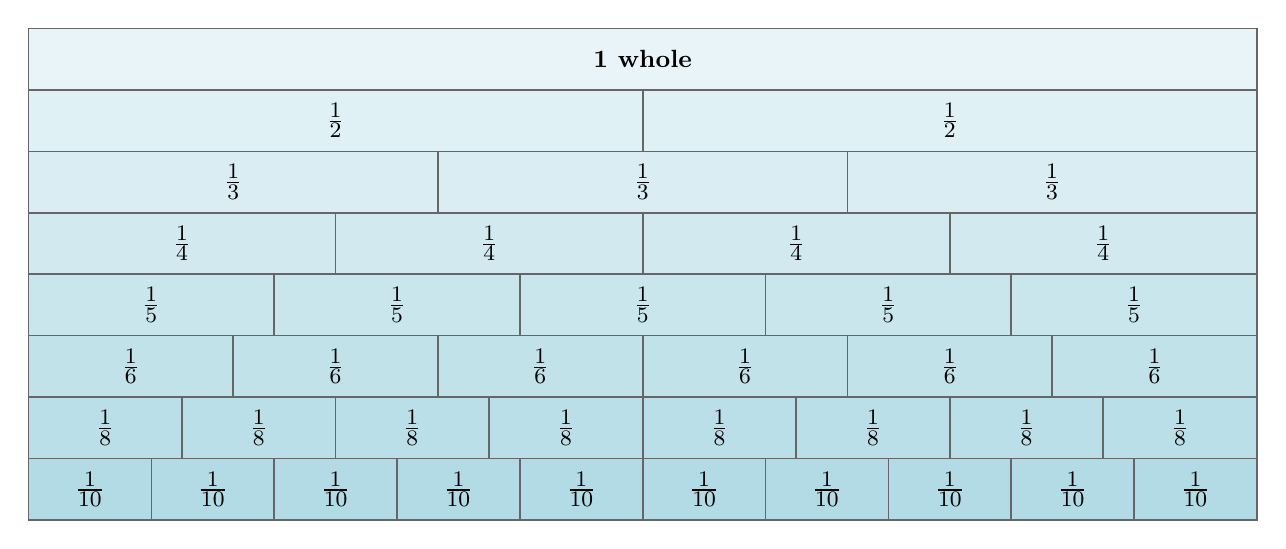
\begin{tikzpicture}[x=1cm, y=1cm]
  \def\W{15.6}
  \foreach \n [count=\r] in {1,2,3,4,5,6,8,10}{%
    \pgfmathsetmacro\w{\W/\n}
    \pgfmathsetmacro\y{-(\r-1)*0.78}
    \foreach \i in {1,...,\n}{%
      \pgfmathsetmacro\x{(\i-1)*\w}
      \filldraw[fill=cbteal!\the\numexpr 6+3*\r\relax, draw=black!60, line width=0.6pt]
        (\x,\y) rectangle ++(\w,0.78);
      \ifnum\n=1
        \node[font=\small\bfseries] at (\x+\w/2,\y+0.39) {1 whole};
      \else
        \node[font=\normalsize] at (\x+\w/2,\y+0.39) {$\tfrac{1}{\n}$};
      \fi}}
\end{tikzpicture}

\vspace{8pt}
\raggedright
{\renewcommand{\arraystretch}{2.3}%
\noindent\begin{tabular}{@{}l@{\ \ }l@{\qquad\qquad}l@{\ \ }l@{\qquad\qquad}l@{\ \ }l@{}}
  \textbf{(a)} & $\fr{1}{2} = \fr{\bxd{2}}{4} = \fr{\bxd{4}}{8}$ &
  \textbf{(b)} & $\fr{1}{3} = \fr{\bx}{6}$ &
  \textbf{(c)} & $\fr{3}{4} = \fr{\bx}{8}$ \\
  \textbf{(d)} & $\fr{2}{3} = \fr{\bx}{6}$ &
  \textbf{(e)} & $\fr{1}{5} = \fr{\bx}{10}$ &
  \textbf{(f)} & $\fr{1}{2} = \fr{\bx}{10}$ \\
\end{tabular}}
\end{minipage}

% -- X4 ---------------------------------------------------------------------
\vfill
\qhead{X4}{Equal or not equal?}

\noindent\begin{minipage}{\textwidth}
\noindent Write $=$ (is equal to) or $\neq$ (is not equal to). Use the fraction wall in X3
to check.

\vspace{6pt}
{\renewcommand{\arraystretch}{2.5}%
\noindent\begin{tabular}{@{}l@{\ \ }l@{\qquad\qquad}l@{\ \ }l@{\qquad\qquad}l@{\ \ }l@{}}
  \textbf{(a)} & $\fr{1}{2} \ \bigcirc\hspace{-0.93em}{\color{cbteal}=}\hspace{0.3em}\ \fr{3}{6}$ &
  \textbf{(b)} & $\fr{2}{3} \ \bigcirc\ \fr{3}{4}$ &
  \textbf{(c)} & $\fr{4}{8} \ \bigcirc\ \fr{1}{2}$ \\
  \textbf{(d)} & $\fr{3}{5} \ \bigcirc\ \fr{6}{10}$ &
  \textbf{(e)} & $\fr{2}{4} \ \bigcirc\ \fr{2}{8}$ &
  \textbf{(f)} & $\fr{2}{3} \ \bigcirc\ \fr{4}{6}$ \\
\end{tabular}}
\end{minipage}

% -- X5 ---------------------------------------------------------------------
\clearpage
\qhead{X5}{Fill the box: follow the arrows}

\noindent\begin{minipage}{\textwidth}
\begin{remember}
  \textbf{Equivalent fractions} show the same amount. Multiply or divide the
  \textbf{top} and the \textbf{bottom} by the \textbf{same number}.
\end{remember}

\noindent\textbf{Multiply.} \ In (b) the arrows are there. In (c) write the number on the
arrow too.

\vspace{4pt}
\noindent\textbf{(a)}\ \eqa{1}{3}{\tl{2}}{\tl{6}}{$\times 2$}\hfill
\textbf{(b)}\ \eqa{2}{5}{\bx}{10}{$\times 2$}\hfill
\textbf{(c)}\ \eqa{3}{4}{\bx}{12}{$\times$\,\bx}\hfill
\textbf{(d)}\ \eqa{5}{6}{10}{\bx}{$\times$\,\bx}
\end{minipage}

\vfill
\noindent\begin{minipage}{\textwidth}
\noindent\textbf{Divide.}

\vspace{4pt}
\noindent\textbf{(e)}\ \eqa{6}{8}{\tl{3}}{\tl{4}}{$\div 2$}\hfill
\textbf{(f)}\ \eqa{9}{12}{3}{\bx}{$\div 3$}\hfill
\textbf{(g)}\ \eqa{10}{15}{\bx}{3}{$\div$\,\bx}\hfill
\textbf{(h)}\ \eqa{8}{10}{\bx}{5}{$\div$\,\bx}
\end{minipage}

\vfill
\noindent\begin{minipage}{\textwidth}
\noindent\textbf{No arrows.} \ You choose the number.

\vspace{4pt}
{\renewcommand{\arraystretch}{3.0}%
\noindent\begin{tabular}{@{}l@{\ \ }l@{\qquad\qquad}l@{\ \ }l@{\qquad\qquad}l@{\ \ }l@{}}
  \textbf{(i)} & $\fr{4}{5} = \fr{\bx}{15}$ &
  \textbf{(j)} & $\fr{1}{6} = \fr{3}{\bx}$ &
  \textbf{(k)} & $\fr{12}{16} = \fr{\bx}{4}$ \\
  \textbf{(l)} & $\fr{2}{7} = \fr{\bx}{14}$ &
  \textbf{(m)} & $\fr{15}{20} = \fr{3}{\bx}$ &
  \textbf{(n)} & $\fr{5}{8} = \fr{\bx}{24}$ \\
  \textbf{(o)} & $\fr{6}{9} = \fr{\bx}{3}$ &
  \textbf{(p)} & $\fr{7}{10} = \fr{\bx}{100}$ &
  \textbf{(q)} & $\fr{18}{24} = \fr{\bx}{4}$ \\
\end{tabular}}

\vspace{6pt}
\vspace{10pt}\noindent\textbf{(r)} Write \textbf{three} fractions that are equal to $\fr{1}{2}$.
\quad\blank[2.0cm]\quad\blank[2.0cm]\quad\blank[2.0cm]
\end{minipage}

% -- X6 ---------------------------------------------------------------------
\clearpage
\qhead{X6}{Count the wholes}

\noindent\begin{minipage}{\textwidth}
\begin{remember}
  \textbf{Improper fraction:} the numerator is bigger than the denominator, like
  $\fr{11}{4}$. It is \textbf{more than 1} whole. \\[4pt]
  \textbf{Mixed number:} a whole number and a fraction, like $\mx{2}{3}{4}$.
\end{remember}

\noindent Mr Bowen's cakes. Count the shaded pieces. Write the amount \textbf{two ways}.

\vspace{6pt}
{\renewcommand{\arraystretch}{1.25}%
\noindent\begin{tabularx}{\textwidth}{@{}l@{\ \ }P{5.6cm}L@{}}
  \textbf{(a)} & \wholes{4}{2}{3} &
    \tl{11} quarters $= \tl{\fr{11}{4}}$ \newline
    \tl{2} wholes and \tl{3} quarters $= \tl{\mx{2}{3}{4}}$ \\[10pt]
  \textbf{(b)} & \wholes{3}{1}{2} &
    \blank[0.9cm] thirds $= \blank[1.3cm]$ \newline
    \blank[0.9cm] whole and \blank[0.9cm] thirds $= \blank[1.3cm]$ \\[10pt]
  \textbf{(c)} & \wholes{2}{3}{1} &
    \blank[0.9cm] halves $= \blank[1.3cm]$ \newline
    \blank[0.9cm] wholes and \blank[0.9cm] half $= \blank[1.3cm]$ \\[10pt]
  \textbf{(d)} & \wholes{5}{2}{1} &
    \blank[0.9cm] fifths $= \blank[1.3cm]$ \newline
    \blank[0.9cm] wholes and \blank[0.9cm] fifth $= \blank[1.3cm]$ \\
\end{tabularx}}
\end{minipage}

% -- X7 ---------------------------------------------------------------------
\vfill
\qhead{X7}{Improper fraction to mixed number: divide}

\noindent\begin{minipage}{\textwidth}
\noindent Divide the top by the bottom. The answer is the \textbf{wholes}. The
\textbf{remainder} goes on top. The bottom stays the same.

\vspace{6pt}
{\renewcommand{\arraystretch}{2.45}%
\noindent\begin{tabular}{@{}l@{\ \ }c@{\quad$\to$\quad}l@{\quad$\to$\quad}l@{}}
  \textbf{(a)} & $\fr{7}{2}$ & $7 \div 2 = \bxd{3}$ \ remainder \ $\bxd{1}$ &
    $\bxd{3}\dfrac{\bxd{1}}{2}$ \\
  \textbf{(b)} & $\fr{9}{4}$ & $9 \div 4 = \bx$ \ remainder \ $\bx$ & $\bx\dfrac{\bx}{4}$ \\
  \textbf{(c)} & $\fr{11}{3}$ & $11 \div 3 = \bx$ \ remainder \ $\bx$ & $\bx\dfrac{\bx}{3}$ \\
  \textbf{(d)} & $\fr{13}{5}$ & $13 \div 5 = \bx$ \ remainder \ $\bx$ & $\bx\dfrac{\bx}{5}$ \\
  \textbf{(e)} & $\fr{17}{6}$ & $17 \div 6 = \bx$ \ remainder \ $\bx$ & $\bx\dfrac{\bx}{6}$ \\
  \textbf{(f)} & $\fr{20}{7}$ & \blank[4.8cm] & \blank[2.0cm] \\
\end{tabular}}

\vspace{4pt}
\noindent\textbf{(g)} $\fr{12}{4}$ \ $= \blank[3.4cm]$ \quad {\small Remainder 0? Then
the answer is just a whole number.}
\end{minipage}

% -- X8 ---------------------------------------------------------------------
\clearpage
\qhead{X8}{Mixed number to improper fraction: multiply, then add}

\noindent\begin{minipage}{\textwidth}
\noindent Multiply the whole number by the bottom. Add the top. The bottom stays the same.

\vspace{6pt}
{\renewcommand{\arraystretch}{2.45}%
\noindent\begin{tabular}{@{}l@{\ \ }c@{\quad$\to$\quad}l@{\quad$\to$\quad}l@{\quad$\to$\quad}l@{}}
  \textbf{(a)} & $\mx{2}{1}{3}$ & $2 \times 3 = \bxd{6}$ & $\bxd{6} + 1 = \bxd{7}$ &
    $\fr{\bxd{7}}{3}$ \\
  \textbf{(b)} & $\mx{1}{3}{4}$ & $1 \times 4 = \bx$ & $\bx + 3 = \bx$ & $\fr{\bx}{4}$ \\
  \textbf{(c)} & $\mx{3}{1}{2}$ & $3 \times 2 = \bx$ & $\bx + 1 = \bx$ & $\fr{\bx}{2}$ \\
  \textbf{(d)} & $\mx{2}{2}{5}$ & $2 \times 5 = \bx$ & $\bx + 2 = \bx$ & $\fr{\bx}{5}$ \\
  \textbf{(e)} & $\mx{4}{1}{3}$ & \blank[2.6cm] & \blank[2.6cm] & \blank[1.4cm] \\
  \textbf{(f)} & $\mx{3}{5}{6}$ & \blank[2.6cm] & \blank[2.6cm] & \blank[1.4cm] \\
\end{tabular}}
\end{minipage}

% -- X9 ---------------------------------------------------------------------
\vfill
\qhead{X9}{On the number line}

\noindent\begin{minipage}{\textwidth}
\noindent Each whole is cut into \textbf{quarters}. Write each letter as a fraction of
quarters \textbf{and} as a mixed number. A is done for you.

\vspace{8pt}
\centering
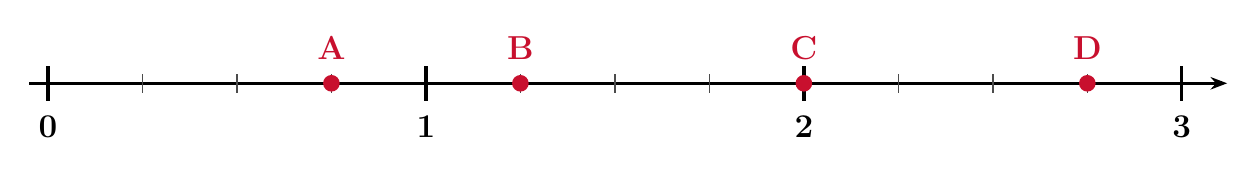
\begin{tikzpicture}[x=4.8cm, y=1cm]
  \draw[line width=1pt, -{Stealth[length=6pt]}] (-0.05,0) -- (3.12,0);
  \foreach \k in {0,...,12} \draw[black!70, line width=0.6pt] (\k/4,-0.12) -- (\k/4,0.12);
  \foreach \k in {0,1,2,3} {
    \draw[line width=1.2pt] (\k,-0.22) -- (\k,0.22);
    \node[below=4pt, font=\large\bfseries] at (\k,-0.15) {\k};}
  \foreach \p/\l in {0.75/A, 1.25/B, 2/C, 2.75/D} {
    \fill[cbred] (\p,0) circle (3pt);
    \node[above=5pt, font=\large\bfseries, text=cbred] at (\p,0) {\l};}
\end{tikzpicture}

\vspace{6pt}
{\renewcommand{\arraystretch}{1.55}%
\begin{tabular}{|C{1.3cm}|C{3.4cm}|C{3.4cm}|}
  \hline
  & \textbf{Quarters} & \textbf{Mixed number} \\ \hline
  A & \tl{$\fr{3}{4}$} & \tl{not more than 1 --- no wholes} \\ \hline
  B \tall & & \\ \hline
  C \tall & & \\ \hline
  D \tall & & \\ \hline
\end{tabular}}
\end{minipage}

% -- X10 --------------------------------------------------------------------
\vfill
\qhead{X10}{Match the pairs}

\noindent\begin{minipage}{\textwidth}
\noindent Draw a line from each improper fraction to the mixed number that is
\textbf{equal}. Be careful: many of them start with 2! The first line is drawn.

\vspace{6pt}
\centering
\begin{tikzpicture}[x=1cm, y=1cm]
  \foreach \t [count=\i] in {{\fr{5}{2}},{\fr{7}{3}},{\fr{9}{4}},{\fr{13}{4}},{\fr{8}{3}},{\fr{10}{3}}} {
    \node[font=\large] at (\i*2.5,0) {$\t$};
    \fill (\i*2.5,-0.75) circle (2.5pt);}
  \foreach \t [count=\i] in {{\mx{3}{1}{3}},{\mx{2}{1}{4}},{\mx{2}{1}{2}},{\mx{2}{2}{3}},{\mx{3}{1}{4}},{\mx{2}{1}{3}}} {
    \node[font=\large] at (\i*2.5,-3.4) {$\t$};
    \fill (\i*2.5,-2.65) circle (2.5pt);}
  \draw[cbteal, line width=1.1pt] (2.5,-0.75) -- (7.5,-2.65);
\end{tikzpicture}
\end{minipage}

% -- X11 --------------------------------------------------------------------
\clearpage
\qhead{X11}{Mr Bowen's fractions}

\begin{wordhelp}
  \eng{a slice / a piece} = one equal part \quad
  \eng{a loaf} = one whole b\'anh m\`i \quad
  \eng{the same amount} = equal
\end{wordhelp}

\noindent\begin{minipage}{\textwidth}
\noindent\textbf{(a)} Mr Bowen cuts a cake into \textbf{8} equal slices. He eats
\textbf{2} slices. What fraction of the cake does he eat? Write it \textbf{two ways}.
\par\vspace{8pt}\hspace*{1.6em}\fbar[6.0]{8}{0}\qquad $\fr{\bx}{8} = \fr{\bx}{4}$
\end{minipage}

\vspace{12pt}
\noindent\begin{minipage}{\textwidth}
\noindent\textbf{(b)} Mr Bowen has $\mx{3}{1}{2}$ pizzas. Each pizza is cut into
\textbf{halves}. How many halves does he have? \ \blank[2.0cm]
\begin{workspace}[2.2cm]{\small\color{black!45} Draw the pizzas if it helps.}\end{workspace}
\end{minipage}

\noindent\begin{minipage}{\textwidth}
\noindent\textbf{(c)} A b\'anh m\`i seller cuts each loaf into \textbf{3} equal pieces.
Mr Bowen buys \textbf{10} pieces. How many loaves is that? Write it as a mixed number.
\ \blank[2.0cm]
\begin{workspace}[2.2cm]\end{workspace}
\end{minipage}

\noindent\begin{minipage}{\textwidth}
\noindent\textbf{(d)} Mr Bowen drinks $\fr{4}{8}$ of a bottle of water. His friend drinks
$\fr{1}{2}$ of the same bottle size. Who drinks more? Circle one.
\par\vspace{6pt}\hspace*{1.6em}Mr Bowen \qquad his friend \qquad they drink
\textbf{the same amount}
\par\vspace{6pt}\hspace*{1.6em}How do you know? \ \blank[9.0cm]
\end{minipage}

% -- X12 --------------------------------------------------------------------
\vfill
\qhead{X12}{Mr Bowen's mistakes}

\noindent\begin{minipage}{\textwidth}
\noindent Mr Bowen did these at home. Tick (\checkmark) the right ones. Cross ($\times$)
the wrong ones and write the correct answer.

\vspace{4pt}
{\renewcommand{\arraystretch}{1.5}%
\noindent\begin{tabularx}{\textwidth}{|C{3.4cm}|C{2.6cm}|L|}
  \hline
  \textbf{His answer} & \textbf{\checkmark\ or $\times$} & \textbf{Correct answer} \\ \hline
  \rule{0pt}{2.2em}$\fr{1}{2} = \fr{2}{3}$ & & \\[6pt] \hline
  \rule{0pt}{2.2em}$\fr{10}{4} = \mx{2}{2}{4}$ & & \\[6pt] \hline
  \rule{0pt}{2.2em}$\mx{2}{1}{5} = \fr{3}{5}$ & & \\[6pt] \hline
  \rule{0pt}{2.2em}$\fr{13}{5} = \mx{3}{2}{5}$ & & \\[6pt] \hline
\end{tabularx}}
\end{minipage}

% ===========================================================================
% PART 2 -- A LITTLE DATA AND KEYS
% ===========================================================================
\clearpage
\hwsection{Part 2 \textperiodcentered\ Data and Keys}

% -- X13 --------------------------------------------------------------------
\qhead{X13}{A word, a count or a measure?}

\noindent\begin{minipage}{\textwidth}
\noindent Tick (\checkmark) one box in each row. (a) is done for you.

\vspace{4pt}
{\renewcommand{\arraystretch}{1.9}%
\noindent\begin{tabularx}{\textwidth}{|L|C{2.3cm}|C{2.3cm}|C{2.3cm}|}
  \hline
  \textbf{Animal fact} & \textbf{a word} & \textbf{a count} & \textbf{a measure} \\[-3pt]
  & {\footnotesize categorical} & {\footnotesize discrete} & {\footnotesize continuous} \\ \hline
  (a) the colour of a parrot & \tl{\checkmark} & & \\ \hline
  (b) the number of legs on a spider & & & \\ \hline
  (c) the mass of a puppy & & & \\ \hline
  (d) the number of eggs in a nest & & & \\ \hline
  (e) where a frog lives: a pond, a river or a rice field & & & \\ \hline
  (f) the length of a snake & & & \\ \hline
\end{tabularx}}
\end{minipage}

% -- X14 --------------------------------------------------------------------
% chicken: legs, feathers. frog: legs, no feathers, no fur. buffalo: legs,
% no feathers, fur/hair. snake: no legs.
\vfill
\qhead{X14}{Use the key}

\noindent\begin{minipage}{\textwidth}
\noindent Start at the top. Answer \textbf{yes} or \textbf{no}. Follow the arrow.
Write the name of each animal. A is done for you.

\vspace{6pt}
\noindent\begin{minipage}[c]{0.56\textwidth}\centering
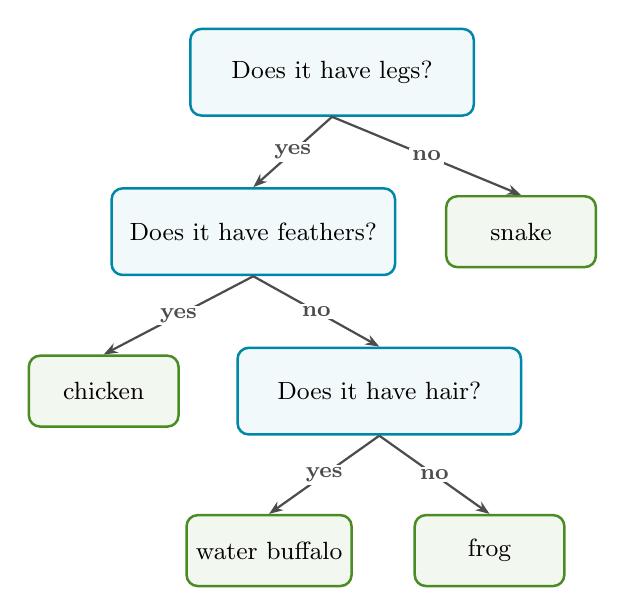
\begin{tikzpicture}[x=1cm, y=1.35cm]
  \node[qbox, minimum width=3.6cm] (q1) at (0,0) {Does it have legs?};
  \node[nbox, minimum width=1.9cm] (snake) at (2.4,-1.5) {snake};
  \node[qbox, minimum width=3.6cm] (q2) at (-1.0,-1.5) {Does it have feathers?};
  \node[nbox, minimum width=1.9cm] (chick) at (-2.9,-3.0) {chicken};
  \node[qbox, minimum width=3.6cm] (q3) at (0.6,-3.0) {Does it have hair?};
  \node[nbox, minimum width=1.9cm] (buff) at (-0.8,-4.5) {water buffalo};
  \node[nbox, minimum width=1.9cm] (frog) at (2.0,-4.5) {frog};
  \draw[br] (q1.south) -- node[yn] {no} (snake.north);
  \draw[br] (q1.south) -- node[yn] {yes} (q2.north);
  \draw[br] (q2.south) -- node[yn] {yes} (chick.north);
  \draw[br] (q2.south) -- node[yn] {no} (q3.north);
  \draw[br] (q3.south) -- node[yn] {yes} (buff.north);
  \draw[br] (q3.south) -- node[yn] {no} (frog.north);
\end{tikzpicture}
\end{minipage}\hfill
\begin{minipage}[c]{0.42\textwidth}
  {\renewcommand{\arraystretch}{1.3}%
  \begin{tabular}{@{}l@{\ \ }P{3.2cm}@{}}
    \textbf{A} & 4 legs, smooth wet skin, no hair. \\
    & Name: \done[2.4cm]{frog} \\[4pt]
    \textbf{B} & No legs. Long body. \\
    & Name: \blank[2.4cm] \\[4pt]
    \textbf{C} & 2 legs. Feathers. \\
    & Name: \blank[2.4cm] \\[4pt]
    \textbf{D} & 4 legs. Hair. Horns. \\
    & Name: \blank[2.4cm] \\
  \end{tabular}}
\end{minipage}
\end{minipage}

% -- X15 --------------------------------------------------------------------
\clearpage
\qhead{X15}{Good question or bad question?}

\noindent\begin{minipage}{\textwidth}
\noindent A \key{good key question}: everyone gives the \textbf{same answer}. Ask about
what you can \textbf{count}, \textbf{measure} or \textbf{see}. Tick good or bad.

\vspace{4pt}
{\renewcommand{\arraystretch}{2.0}%
\noindent\begin{tabularx}{\textwidth}{|L|C{2.0cm}|C{2.0cm}|}
  \hline
  \textbf{Key question} & \textbf{good} & \textbf{bad} \\ \hline
  (a) Does it have wings? & \tl{\checkmark} & \\ \hline
  (b) Is it cute? & & \\ \hline
  (c) Is it big? & & \\ \hline
  (d) Does it have more than 4 legs? & & \\ \hline
  (e) Is it scary? & & \\ \hline
  (f) Is it longer than 1 m? & & \\ \hline
\end{tabularx}}
\end{minipage}

% -- X16 --------------------------------------------------------------------
% fish: no legs. butterfly: 6 legs. chicken: 2 legs, feathers. dog: 4 legs, fur.
\vfill
\qhead{X16}{Finish the key}

\noindent\begin{minipage}{\textwidth}
\noindent Four animals: \textbf{fish}, \textbf{butterfly}, \textbf{chicken},
\textbf{dog}. Write the two missing questions and the three missing names. Use the
word bank.

\vspace{4pt}
\noindent\textbf{Word bank:} \quad \fbox{6 legs} \quad \fbox{feathers} \quad
\fbox{butterfly} \quad \fbox{chicken} \quad \fbox{dog}

\vspace{8pt}
\centering
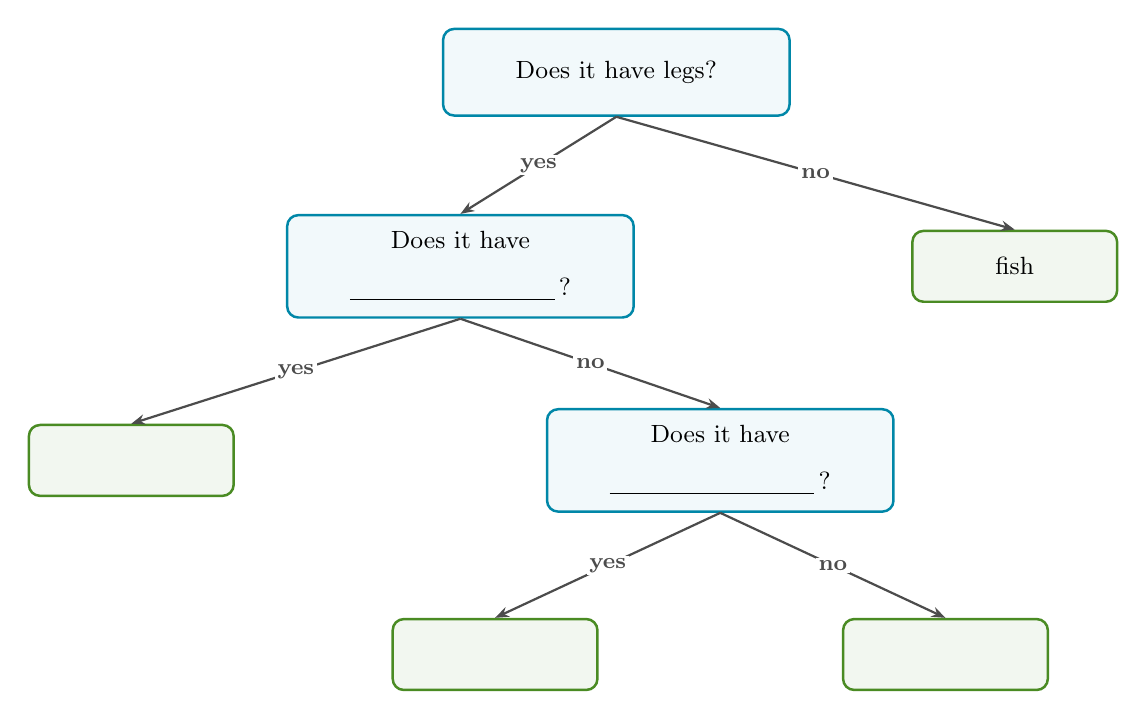
\begin{tikzpicture}[x=1.1cm, y=1.45cm]
  \node[qbox] (q1) at (0,0) {Does it have legs?};
  \node[nbox] (fish) at (4.6,-1.7) {fish};
  \node[qbox, minimum height=1.3cm] (q2) at (-1.8,-1.7) {Does it have \\[6pt]
    \blank[2.6cm]\,?};
  \node[nbox] (n1) at (-5.6,-3.4) {};
  \node[qbox, minimum height=1.3cm] (q3) at (1.2,-3.4) {Does it have \\[6pt]
    \blank[2.6cm]\,?};
  \node[nbox] (n2) at (-1.4,-5.1) {};
  \node[nbox] (n3) at (3.8,-5.1) {};
  \draw[br] (q1.south) -- node[yn] {no} (fish.north);
  \draw[br] (q1.south) -- node[yn] {yes} (q2.north);
  \draw[br] (q2.south) -- node[yn] {yes} (n1.north);
  \draw[br] (q2.south) -- node[yn] {no} (q3.north);
  \draw[br] (q3.south) -- node[yn] {yes} (n2.north);
  \draw[br] (q3.south) -- node[yn] {no} (n3.north);
\end{tikzpicture}
\end{minipage}

% ===========================================================================
% ANSWER KEY -- TEACHER COPY ONLY
% ===========================================================================
\ifkey
\clearpage

\hwsection[cbred]{Answer Key --- Teacher Copy}

\linespread{1.0}\selectfont
\setlist[enumerate]{itemsep=2pt, topsep=3pt, leftmargin=*}

\qhead[cbred]{X1}{What fraction is shaded?}
\noindent (b) $\fr{1}{4}$ one quarter \quad (c) $\fr{2}{5}$ two fifths \quad
(d) $\fr{5}{6}$ five sixths \quad (e) $\fr{7}{10}$ seven tenths

\smallskip
\noindent{\small Expect $\fr{1}{3}$ for (b) (shaded : not shaded, 1 to 3) --- the
denominator is \emph{all} the parts. ``Five six'' for (d): the word help gives the
pattern; ``sixths'' is the word to hear.}

\qhead[cbred]{X2}{Shade the same amount}
\noindent (b) $\fr{2}{6}$ \quad (c) $\fr{6}{8}$ \quad (d) $\fr{4}{10}$

\smallskip
\noindent{\small The student shades until the edge lines up with the top bar. A student
who shades 3 of 8 in (c) copied the numerator; ask them to put a ruler down the edge of
the top bar.}

\qhead[cbred]{X3}{The fraction wall}
\noindent (b) 2 \quad (c) 6 \quad (d) 4 \quad (e) 2 \quad (f) 5

\qhead[cbred]{X4}{Equal or not equal?}
\noindent (b) $\neq$ \quad (c) $=$ \quad (d) $=$ \quad (e) $\neq$ \quad (f) $=$

\smallskip
\noindent{\small (e) is the trap: the same numerator, so ``equal''. On the wall
$\fr{2}{8}$ is half of $\fr{2}{4}$.}

\qhead[cbred]{X5}{Fill the box}
\noindent (b) $\fr{4}{10}$ \quad (c) $\times 3$, $\fr{9}{12}$ \quad
(d) $\times 2$, $\fr{10}{12}$ \quad (f) $\fr{3}{4}$ \quad (g) $\div 5$, $\fr{2}{3}$
\quad (h) $\div 2$, $\fr{4}{5}$ \quad (i) $\fr{12}{15}$ \quad (j) $\fr{3}{18}$ \quad
(k) $\fr{3}{4}$ \quad (l) $\fr{4}{14}$ \quad (m) $\fr{3}{4}$ \quad
(n) $\fr{15}{24}$ \quad (o) $\fr{2}{3}$ \quad (p) $\fr{70}{100}$ \quad (q) $\fr{3}{4}$
\quad (r) any three of $\fr{2}{4}, \fr{3}{6}, \fr{4}{8}, \fr{5}{10}, \ldots$

\smallskip
\noindent{\small (c): ``4 to 12 is $\times 3$'' --- find the arrow from the number you
have. Expect $\fr{11}{12}$ from adding 8 to both. (k) can be done in two steps
($\div 2$, $\div 2$).}

\qhead[cbred]{X6}{Count the wholes}
\noindent (b) 5 thirds $= \fr{5}{3}$; 1 whole and 2 thirds $= \mx{1}{2}{3}$ \quad
(c) 7 halves $= \fr{7}{2}$; 3 wholes and 1 half $= \mx{3}{1}{2}$ \quad
(d) 11 fifths $= \fr{11}{5}$; 2 wholes and 1 fifth $= \mx{2}{1}{5}$

\smallskip
\noindent{\small Expect $\fr{5}{4}$ in (b) from counting pieces and cakes (5 pieces, 4
\ldots). The bottom is the number of pieces in \emph{one} cake.}

\qhead[cbred]{X7}{Improper to mixed}
\noindent (b) 2 r 1, $\mx{2}{1}{4}$ \quad (c) 3 r 2, $\mx{3}{2}{3}$ \quad
(d) 2 r 3, $\mx{2}{3}{5}$ \quad (e) 2 r 5, $\mx{2}{5}{6}$ \quad
(f) $20 \div 7 = 2$ r 6, $\mx{2}{6}{7}$ \quad (g) 3

\smallskip
\noindent{\small The common slip is putting the answer on top and the remainder in
front ($\mx{1}{2}{4}$ for (b)). Point at (a): the \emph{wholes} come first.}

\qhead[cbred]{X8}{Mixed to improper}
\noindent (b) 4, 7, $\fr{7}{4}$ \quad (c) 6, 7, $\fr{7}{2}$ \quad (d) 10, 12,
$\fr{12}{5}$ \quad (e) $4 \times 3 = 12$, $12 + 1 = 13$, $\fr{13}{3}$ \quad
(f) $3 \times 6 = 18$, $18 + 5 = 23$, $\fr{23}{6}$

\smallskip
\noindent{\small Expect ``forgot to add'' ($\fr{12}{3}$ in (e)) and ``added the whole''
($\fr{5}{3}$ in (e): $4 + 1$).}

\qhead[cbred]{X9}{On the number line}
\noindent B $\fr{5}{4} = \mx{1}{1}{4}$ \quad C $\fr{8}{4} = 2$ \quad
D $\fr{11}{4} = \mx{2}{3}{4}$

\smallskip
\noindent{\small C is a whole number: 8 quarters are 2 wholes. Students who count the
big marks as quarters will write $\fr{2}{4}$ for C.}

\qhead[cbred]{X10}{Match the pairs}
\noindent $\fr{5}{2} = \mx{2}{1}{2}$ \quad $\fr{7}{3} = \mx{2}{1}{3}$ \quad
$\fr{9}{4} = \mx{2}{1}{4}$ \quad $\fr{13}{4} = \mx{3}{1}{4}$ \quad
$\fr{8}{3} = \mx{2}{2}{3}$ \quad $\fr{10}{3} = \mx{3}{1}{3}$

\qhead[cbred]{X11}{Mr Bowen's fractions}
\noindent (a) $\fr{2}{8} = \fr{1}{4}$ \quad (b) 7 halves \quad
(c) $\fr{10}{3} = \mx{3}{1}{3}$ loaves \quad (d) the same amount: $\fr{4}{8} = \fr{1}{2}$

\smallskip
\noindent{\small (b) Expect 6 (they forgot the half pizza) or 3.5. (d) is the
``bigger numbers, bigger fraction'' error: expect ``Mr Bowen, because 4 is bigger than
1''.}

\qhead[cbred]{X12}{Mr Bowen's mistakes}
\noindent Row 1 $\times$: $\fr{1}{2} = \fr{2}{4}$ (he added 1). \quad Row 2
\checkmark\ ($= \mx{2}{1}{2}$ too). \quad Row 3 $\times$: $\fr{11}{5}$ (he added 2 and 1).
\quad Row 4 $\times$: $\mx{2}{3}{5}$ (he swapped the wholes and the remainder).

\qhead[cbred]{X13}{A word, a count or a measure?}
\noindent (b) count \quad (c) measure \quad (d) count \quad (e) word \quad (f) measure

\qhead[cbred]{X14}{Use the key}
\noindent B snake \quad C chicken \quad D water buffalo

\qhead[cbred]{X15}{Good question or bad question?}
\noindent (b) bad \quad (c) bad \quad (d) good \quad (e) bad \quad (f) good

\smallskip
\noindent{\small (c) and (f) are the pair to talk about: ``big'' is different for
everyone; ``longer than 1 m'' is a measure.}

\qhead[cbred]{X16}{Finish the key}
\noindent Question 2: Does it have \textbf{6 legs}? Yes: \textbf{butterfly}. \quad
Question 3: Does it have \textbf{feathers}? Yes: \textbf{chicken}; No: \textbf{dog}.

\smallskip
\noindent{\small Accept Question 2 ``feathers'' if the names follow it (yes: chicken;
then ``6 legs'': butterfly / dog). Check that every name appears once.}
\fi

\end{document}
